\documentclass[10pt, a4paper]{exam}
\usepackage{graphicx}
\usepackage[a4paper, total={7in, 9.5in}]{geometry}
\usepackage[normalem]{ulem}
\usepackage{amsmath}
\renewcommand\ULthickness{1.0pt}   
\setlength\ULdepth{1.3ex}

\begin{document}


	\noindent
	\begin{minipage}[l]{0.1\textwidth}
		\noindent
		
\includegraphics[width=2.8\textwidth]{ESCUDO.png}
	\end{minipage}
\hfill
\begin{minipage}[c]{0.8\textwidth}
	\begin{center}
		{\large  Departamento de Ingeniería civil y Agrícola\par
		\large	Facultad de Ingeniería	\par
	% \large \textbf{Taller propiedades de los fluidos}	\par
    \large \textbf{Laboratorio No. 2\\Compuerta}	\par
} %%%%% NOMBRE DEL PROFESOR 
	\end{center}
\end{minipage}
\par
\vspace{0.2in}
\noindent
    \uline{Estructuras hidráulicas [2015954]	\hfill 2024-II	}
\par 
\vspace{0.15in}
\noindent

%%%%%%%%%%%%%%%%%%%%%%%%%%%%%
\section{Normas del Laboratorio}
\begin{itemize}
    \item \textbf{Grupos}: Los grupos serán de 5 o 6 estudiantes máximo. Los estudiantes son libres de organizar los grupos.
    
    \item \textbf{Duración}: Cada grupo tendrá una hora aproximadamente para realizar el laboratorio.
    
    \item \textbf{Material}: Es necesario vestir bata u overol para la realización del laboratorio. Este atuendo puede ser de cualquier color o fabricante. Traer calculadora, lápiz y papel.
\end{itemize}


\section{Objetivo}

En términos generales, este laboratorio tiene como fin estudiar el flujo a través de una compuerta y otros parámetros debido a la misma.

\begin{itemize}

    \item Analizar los coeficientes de descarga $(C_d)$ y contracción $(C_c)$ en una compuerta, manteniendo una apertura fija.
    
    \item Examinar cómo se distribuyen las presiones y las velocidades a lo largo de la longitud del canal y en la superficie de la compuerta.
    
\end{itemize}


\section{Metodología}

Se dispondrá de un canal rectangular de paredes de vidrio de $31cm$ de ancho, dicho canal se alimenta mediante un tanque de aquietamiento al conecta una tubería proveniente de un tanque de nivel constante, el caudal a utilizar se regula mediante una válvula colocada en la tubería. \vspace{1ex}

El tanque volumétrico será utilizado para el cálculo del caudal que pasara por la compuerta, este valor se conoce midiendo el desplazamiento de la cinta y el tiempo que transcurre en dicho desplazamiento (Figura \ref{fig:cinta}). 


\begin{figure}[h]
    \centering
    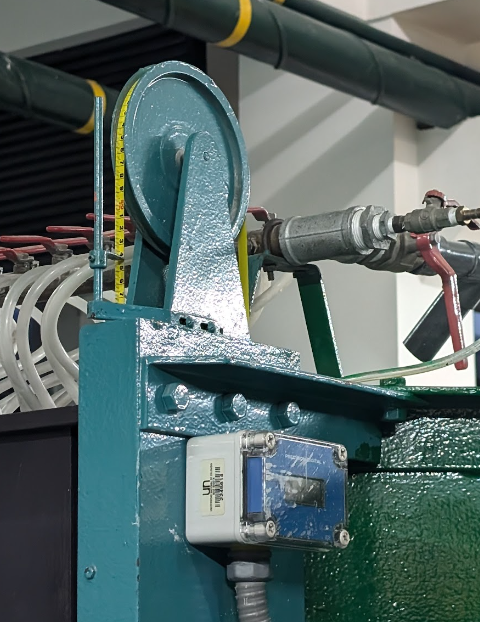
\includegraphics[width=0.29\linewidth]{Images/cinta.png}
    \caption{Cinta para la medición del caudal.}
    \label{fig:cinta}
\end{figure}

\newpage

A lo largo del canal se encuentra un limnímetro montado en un riel desplazable a lo largo del canal, este instrumento será el que permitirá las medidas de las profundidades a lo largo del canal. El esquemático del montaje anterior se evidencia en las imágenes \ref{fig:esqpdf}.

\begin{figure}[h]
    \centering
    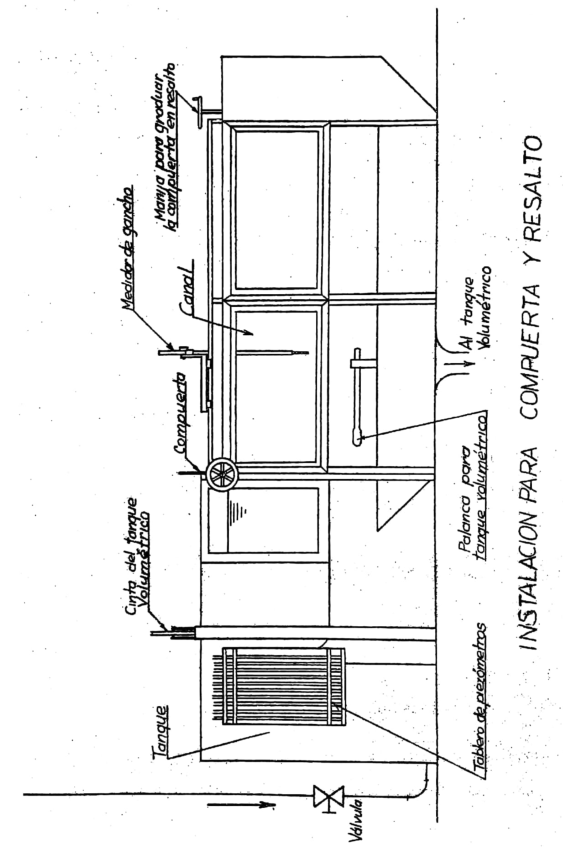
\includegraphics[angle=270,width=0.6\linewidth]{Images/esquema.png}
    \caption{Esquema general de la instalación.}
    \label{fig:esqpdf}
\end{figure}

Además, se tiene una compuerta colocada después del tanque de aquietamiento sobre el canal y un tablero de piezómetros provenientes del fondo del canal y de la pared de la compuerta. Dicha distribución de piezómetros se muestra más claramente en la figura \ref{fig:piezo}.

\begin{figure}[h]
    \centering
    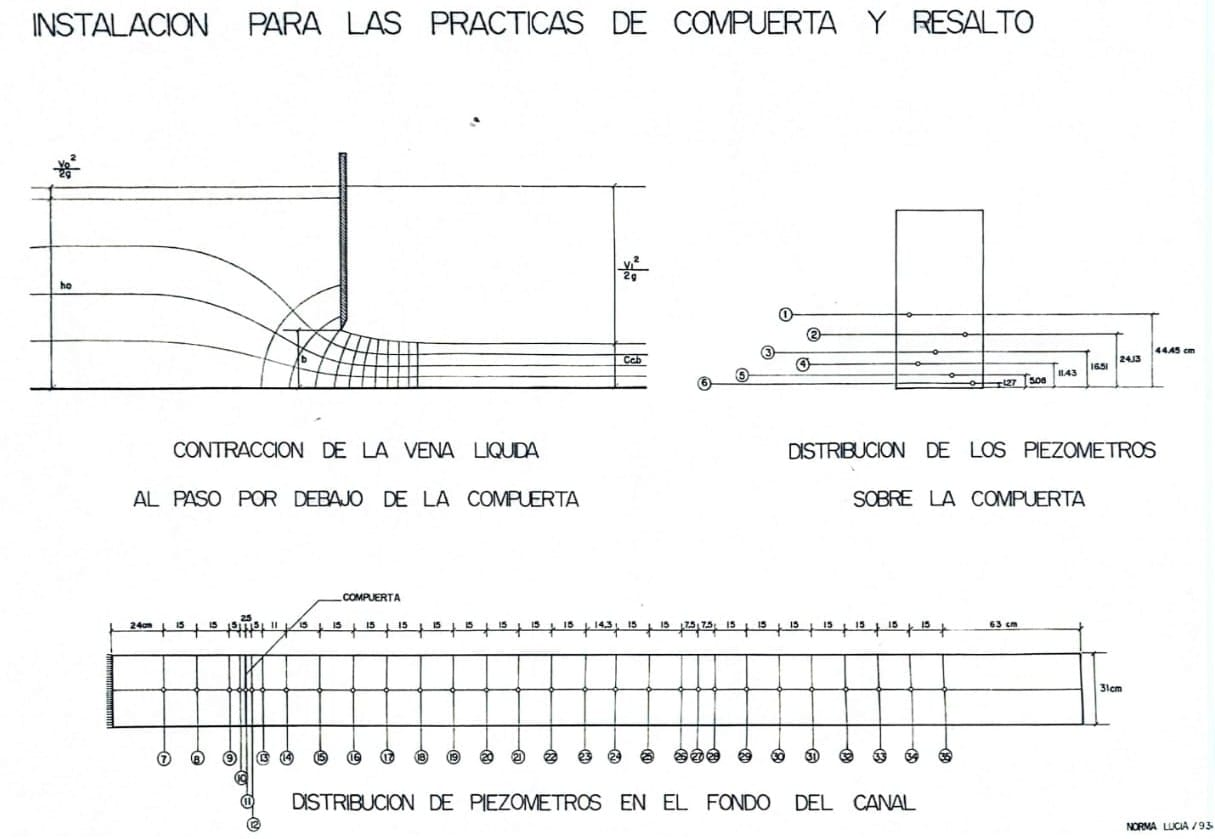
\includegraphics[width=0.76\linewidth]{Images/piezo.jpg}
    \caption{Distribución de piezómetros en el fondo y en la compuerta del canal.}
    \label{fig:piezo}
\end{figure}

\newpage

\begin{figure}[h]
    \centering
    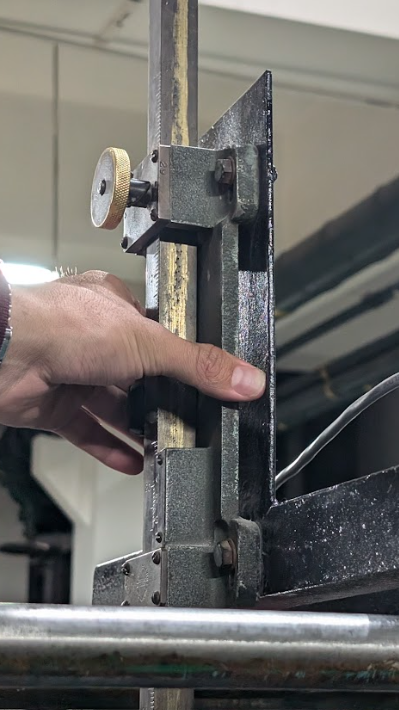
\includegraphics[width=0.3\linewidth]{Images/limnimetro.png}
    \caption{Limnímetro a utilizar para la medición de la lámina de agua.}
    \label{}
\end{figure}

\begin{figure}[h]
    \centering
    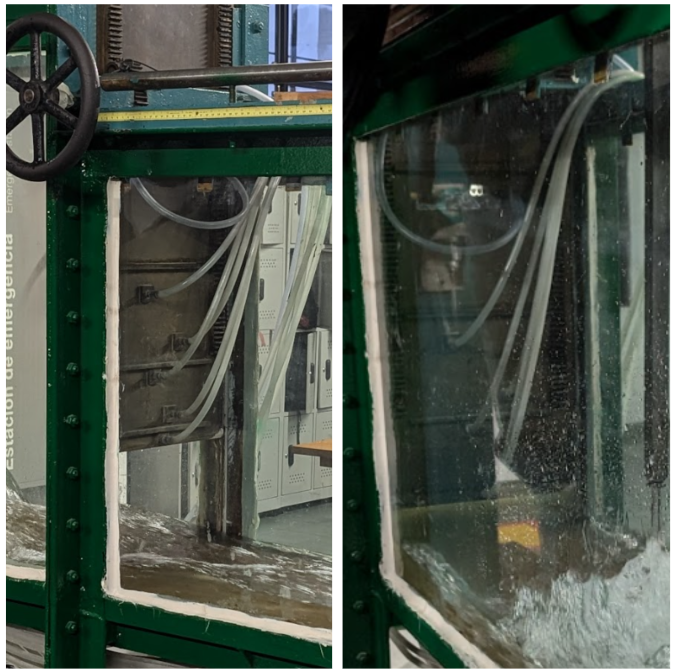
\includegraphics[width=0.38\linewidth]{Images/compuer2.png}
    \caption{Compuerta aguas arriba utilizada en la práctica.}
    \label{}
\end{figure}


\newpage

\section{Ecuaciones y resultados}


\begin{enumerate}

    \item Teniendo como planteamiento del siguiente esquema, para obtener el caudal por unidad de ancho aplicamos Bernoulli en las dos secciones del flujo, obteniendo:

    \begin{figure}[h]
        \centering
        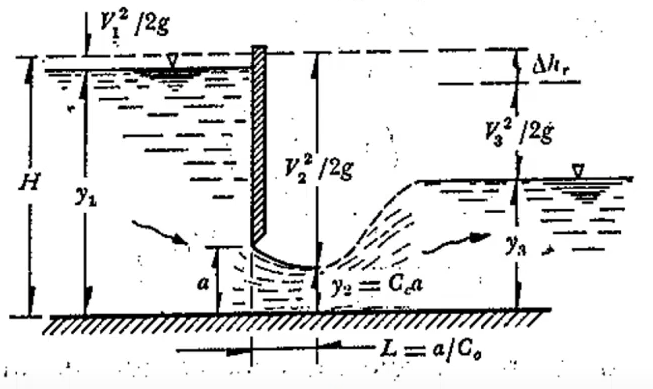
\includegraphics[width=0.5\linewidth]{Images/compuer.png}
        \caption{Esquema de flujo para la compuerta.}
        \label{}
    \end{figure}

    $$y_1+\dfrac{v^2_1}{2g}=\dfrac{v^2_2}{2g}+y_2$$
    $$y_1+\dfrac{v^2_1}{2g}=\dfrac{v^2_2}{2g}+C_c \cdot a$$
    $$q=v_1\cdot y_1=v_2\cdot C_c \cdot a$$

    Se tiene entonces que:

    $$q=\dfrac{C_c}{\sqrt{1+Cc \cdot\dfrac{a}{y_1}}}\cdot a \cdot  \sqrt{2gy_1}$$

    Es así que, introduciendo el coeficiente de descarga se tiene:

    $$q=C_d \cdot a \cdot \sqrt{2gy_1}$$ 

    O en términos del caudal, donde $B$ corresponde al ancho del canal

    $$Q=C_d \cdot a \cdot B \cdot \sqrt{2gy_1}$$ 

    Donde $C_d$ corresponde a:

    $$C_d=\dfrac{C_c}{\sqrt{1+Cc \cdot\dfrac{a}{y_1}}}$$

    Note que si despejamos $C_c$ en función del coeficiente de descarga se puede obtener la siguiente expresión:

    $$C_c=C_d+\dfrac{Cd^2}{2}\cdot\dfrac{a}{y_1}$$

    \item Calcular los coeficientes de descarga $(C_d)$ y de contracción $(C_c)$ para los diferentes caudales empleados en la práctica a partir de las mediciones experimentales promediando las alturas medidas para un mismo caudal.
    
    \item Determinar aproximadamente, el coeficiente de contracción $(C_c)$ para la compuerta, dividiendo la profundidad mínima del agua en el canal $(y_2)$ por la abertura de la compuerta $a$ (esto con ayuda del limnímetro o cualquier otro instrumento que le permita medir la altura).

    
    \item Comparar y explicar las posibles diferencias de los valores obtenidos en (2) y (3) con el valor teórico de $C_c=0.611$

    
    \item Dibujar en papel milimetrado, tomando como ejes de referencia el fondo del canal y la compuerta, las gráficas correspondientes de distribución de presiones a lo largo del fondo del canal y de la pared de la compuerta. Dibujar para el mayor caudal. 

    
    \item Dibujar el perfil de la superficie libre antes y después de la compuerta, así como la línea de energía para el caudal del punto anterior.

    \item Mediante la aplicación de la Ecuación de Bernoulli demostrar en base a los valores de la experiencia, que la pérdida de energía a través de la compuerta es muy pequeña.

    \item Calcular la fuerza total sobre la compuerta a partir de la distribución de presiones hallada.

    \item Calcular la fuerza $F$ sobre la compuerta por aplicación de la Ecuación de cantidad de movimiento:

    $$B\cdot\gamma\left(\frac{y_1}{2} - \frac{(C_c \cdot a)^2}{2}\right) - F = Q \cdot \frac{\gamma}{g} \left(v_2-v_1 \right)$$

    Donde: 

    \begin{itemize}
        \item $\gamma$ = Peso específico del agua $(1gr/cm^3)$.
        \item $B$ = Ancho del canal.
    \end{itemize}
\end{enumerate}


\section{Listado de instrumentos usados}

\begin{enumerate}

    \item Medición de caudal y presión:
    
        \begin{enumerate}
        
            \item \textbf{Tanque volumétrico:} Utilizado para medir el caudal.

            \item \textbf{Tablero de piezómetros:} Instrumentos utilizados para medir la presión del agua.
            
        \end{enumerate}
        
    \item Medición y control de altura:
    
        \begin{enumerate}
        
            \item \textbf{Compuertas:} Utilizadas aguas arriba y aguas abajo del canal para regular el flujo.
            \item \textbf{Limnímetro:} Conjunto de reglas graduadas en centímetros que miden las variaciones del nivel de la superficie del agua.
            
        \end{enumerate}
        
\end{enumerate}

\section{Informe}

El informe de laboratorio debe contener las siguientes secciones:

\begin{enumerate}

    \item \textbf{Introducción:} Breve texto para poner en contexto el laboratorio.
    
    \item \textbf{Metodología:} Describe el procedimiento de toma de datos y el seguido para obtener los resultados (sustentar con algunas fotografías de ser posible).
    
    \item \textbf{Resultados y análisis:} Presenta los resultados del laboratorio. Dado el caso, se deben incluir gráficas y tablas que resuman los resultados.
    
    \item \textbf{Conclusiones:} Se discuten allí las conclusiones obtenidas a partir de los resultados. Se hacen las comparaciones del caso.
    
    \item \textbf{Referencias:} Incluir las referencias consultadas.
\end{enumerate}


\end{document}



